\section{Introduction}
\label{sec:introduction}

\IEEEPARstart{C}{ervical} cancer is the second most common gynecological tumor worldwide, and the fourth leading cause of cancer-related death in women. Early diagnosis and intervention have been recognized as an effective way to manage cervical cancer, while delayed diagnosis will have a much negative impact on the patient's prognosis and may even lead to mortality. In this way, large-scale screening is considered as pivotal worldwide for the prevention and in-time administration of cervical abnormality~\cite{schiffman2007human}.



Nowadays, thin-prep cytologic test (TCT) is widely-applied for cervical cancer screening~\cite{koss1989papanicolaou}. 
Compared to the early technique of pap smear, TCT uses machine filtration to evenly disperse the cells and removes the interference of impurities. The TCT examinations generally follow the Bethesda System (TBS)~\cite{nayar2015bethesda}, which categorizes the cervical cells into the following types: normal class or negative for intraepithelial malignancy (NILM), atypical squamous cells (ASC), low-grade squamous intraepithelial lesion (LSIL), and high-grade squamous intraepithelial lesion (HSIL). 
Fig. \ref{fig:tbs} presents examples of cervical cells in different types. 
Generally, NILM stands for the normal or \textit{negative} samples, while the rests are \textit{positive} in different degrees and require follow-up examinations. 



\begin{figure}
    \centering
    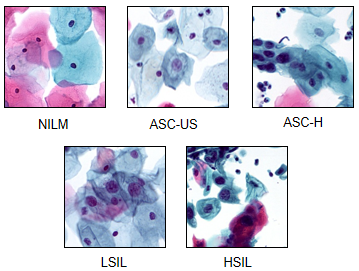
\includegraphics[scale=0.8]{figures/tbs.png}
    \caption{Examples of cervical cells in different degrees: NILM is the ``normal'' case, while the rest are abnormal types, and ASC-H, LSIL and HSIL are the advanced abnormal types indicating a more severe progression of symptoms.}
    \label{fig:tbs}
\end{figure}


Conventional TCT examinations are implemented by visual inspection of the stained samples with collected cervical cells under the microscope, which requires substantial expertise from pathologists and becomes a challenging problem worldwide. It can be observed from Fig. \ref{fig:tbs} that the differentiation of different cervical cell types is subtle in appearance and morphometry. And pathologists rely on key (abnormal) cells to make diagnoses. Especially in the low-middle income areas where healthcare resources are limited, the screening needs are relatively more challenging for pathologists to handle. Therefore, a fully automatic computer-aided diagnosis (CAD) system is highly desired for TCT screening, which is implemented based on the scanned whole-slide images (WSIs) and completes the screening in a high-throughput and robust way.




Recently, deep learning has emerged as a promising tool for the automatic diagnosis of many diseases. 
In the field of pathology, the screening of cervical abnormalities has drawn a lot of attention. Due to the image size of the scanned WSIs which are generally huge (e.g. normally about $30000\times 40000$ in image size for a WSI sample under study), the CAD system for WSI screening is usually implemented in a hierarchical manner. 



% Generally speaking, concerning the complexity of the screening task, deep learning methods usually solve this problem step by step. 
For example, Zhou et al. \cite{zhou2021hierarchical} proposed a three-step framework for TCT screening.
First, a cell detection network is trained to localize the suspicious abnormal cervical cells from WSI.
Then, the patch is center-cropped for each suspicious cell, and further processed through a classification model to tell whether the patch is positive or negative. 
Finally, the typical positive patches determined by the patch-level classification are further ensembled, such that the overall positive/negative diagnosis is produced for the WSI at the sample level. 

Similar ideas are also shared by several related works in the literature.
Cao et al. \cite{cao2021novel} proposed the cell detection model of AttFPN, which benefited from the clinical knowledge and the attention mechanism, to improve the detection performance. Cheng et al.
\cite{cheng2021robust} proposed a progressive identification method that combined multi-scale visual cues to identify abnormal cells, and a recurrent neural network (RNN) was adopted to complete the sample-level classification based on the patches cropped from the abnormal cells. Wei et al. \cite{wei2021efficient} proposed the cervical screening method which focused on improving both the cell detection network and the classification network. They adopted the YOLO architecture and added a variety of convolution kernels of different sizes to adapt to the highly diverse cell clusters, and they also used the transformer to improve classification performance.


% \todo{What is the limitation of existing methods or the challenge unresolved yet? You need summarize the problems first, then propose your method solve the problems.}

Although many works have contributed to TCT screening, there are still several challenges that remain unsolved: 

\begin{itemize}
    \item 
   The differentiation of cervical cells in TCT examinations is challenging even for professional pathologists. 
   And the classification is quite subjective although the TBS specifications illustrate the cervical cell abnormality in different types. There are unavoidable cell sets that cannot be easily recognized by the pathologists, which are recognized as the \textit{hard} samples in our work\todo{I don't think it's correct here. We didn't use pathologist labeling to identify hard samples}. As the \textit{ground-truth} labels of those cells are not fully convincing, they need to be handled in a specific manner when constructing the learning-based classifiers.
    \item 
    As the CAD-based TCT examinations are generally implemented in a hierarchical manner, the WSI-level classification needs to be implemented based on the aggregation of the detected suspicious cell results. The ensembling strategy needs to be spatially dynamic, as individual cells from different locations may have evidence of varying strength to support the sample-level decision.
    \item 
    Finally, the screening system should be highly sensitive overall, such that false negatives can be mostly suppressed and cervical abnormality can raise alert as early as possible. 
    Therefore, the sample-level decision is usually ensembled from a relatively large number of cell patches per WSI (e.g., 20 in our implementation), in case the cell detection may not identify those positive cells if the number is too small \cite{zhou2021hierarchical}. 
    Contrarily, those patches often have similar appearances. And even for a positive sample, the to-be-ensembled patches may have appearances that are close to negative. Thus, one may need to pay special attention to suppressing the redundant and distorting patches when ensembling them.
\end{itemize}


To solve the problems above, here we propose a novel TCT screening framework that effectively combines traditional convolutional neural network (CNN) and transformer structure, aiming at improving the sample-level classification performance through the powerful local feature extraction capability of CNN, and the global feature fusion capability of the transformer structure. We also propose a novel clustering loss\todo{Still clustering loss?} to improve the capacity of feature representation for our patch-level CNN model. For sample-level classification, we propose a novel score embedding and hierarchical token aggregation strategy to deal with different patches within the sample. The main contributions of our work are listed as follows:  




\begin{itemize}
    \item We design a novel TCT screening framework, which combines CNN and transformer to further fuse global features on the basis of effectively extracted local features, 
    and improve classification on sample-level for cervical cancer screening.
    \item We design a novel patch-level image feature extraction strategy from the CNN network, using the hard patches mining method to make the feature space more compact and reasonable. Thus, the model can have a stronger ability to distinguish hard patches.
    \item We design the classification scores for each patch and treat these scores as unique location information in the feature space to have a score embedding for each patch, thus allowing the transformer model to better exploit the relationship between different patches.
    \item We develop a novel token pooling strategy with the tokens input into the transformer to simplify more representative tokens, so that the network can learn which tokens to pay attention to, and ultimately improve the classification effect.
\end{itemize}

The rest of this paper is organized as follows, Section \ref{sec:related} is the related works, which contains the common structures in medical images and the common methods for feature-based learning. Then in Section \ref{sec:method} we introduce our proposed method, which mainly consists of the patch-level classification model and the sample-level classification model. In Section \ref{sec:experiments} we conduct experiments to both evaluate the effectiveness on the patch-level and sample-level, and finally the related discussions and conclusions presented in Section \ref{sec:discussion} and Section \ref{sec:conclusion}, respectively.

